% !TeX spellcheck = es_ES
\documentclass[12pt, titlepage]{article}
\usepackage[letterpaper, margin=2.5cm]{geometry}
\usepackage[utf8]{inputenc}
\usepackage[spanish]{babel}

\usepackage{amsmath}

\usepackage{float}
\usepackage{graphicx}

\usepackage{color}
\usepackage{listings}
\usepackage[nottoc,notlot,notlof]{tocbibind}
\definecolor{dkgreen}{rgb}{0,0.6,0}
\definecolor{gray}{rgb}{0.5,0.5,0.5}
\definecolor{mauve}{RGB}{253,151,31}
\definecolor{deepred}{RGB}{249,38,114}
\lstset{frame=tb,
language=Python,
aboveskip=3mm,
belowskip=3mm,
showstringspaces=false,
columns=flexible,
numbers=left,
stepnumber=1,
basicstyle={\small\ttfamily},
numberstyle=\tiny\color{gray},
keywordstyle=\color{blue},
commentstyle=\color{dkgreen},
stringstyle=\color{mauve},
breaklines=true,
breakatwhitespace=true,
tabsize=2,
morekeywords={self, append},
emph={Transicion, __init__, True, False, __str__, AFN, AFD, Analizador, var, 
asig, Prueba, mayorque, menorque, sumar, restar, eof},
emphstyle=\color{deepred}
}

%opening
\title{Reporte: Práctica 5}
\author{Barrera Pérez Carlos Tonatihu \\ Profesor: Saucedo Delgado Rafael 
Norman 
\\ Compiladores \\ Grupo: 3CM6}

\begin{document}

\maketitle
\tableofcontents
\newpage
\section{Introducción}
Un analizador por descenso recursivo es un analizador sintáctico de arriba hacia abajo en el cual un conjunto de métodos recursivos son usados para procesar una entrada.
El análisis de arriba hacia abajo puede ser visto como un intento de encontrar la derivación mas a la izquierda para una cadena.
Esto genera que el árbol de sintaxis sea construido desde la raíz y creando nodos en preorden. \cite{compis}

En este tipo de analizador se tiene un método asociado a cada símbolo no 
terminal de la gramática.
\newpage
\section{Desarrollo}
Se desarrollo un analizador sintáctico por descenso recursivo para un lenguaje 
bastante sencillo cuyas principales características son:
\begin{itemize}
 \item Declaración de variables.
 \item Asignación de variables.
 \item Operaciones binarias (suma, resta, operaciones lógicas).
 \item Comparaciones (\emph{if}).
 \item Ciclos (\emph{while}).
 \item Fin de archivo con la palabra reservada \emph{eof}.
 \item Fin de declaración de instrucción con punto y coma.
\end{itemize}
Es por esto que se tuvo que hacer un analizador léxico para reconocer este 
lenguaje, este analizador fue realizado utilizando la herramienta PLY. El 
código del analizador léxico es el siguiente.
\begin{lstlisting}
tokens = [
    'p',
    'q',
    'c',
    'z',
    'a',
    'n',
]
palabras_reservadas = {
    'if': 'i',
    'while': 'l',
    'var': 'v',
    'asig': 'b',
    'sumar': 'o',
    'mayorque': 'm',
    'restar': 'o',
    'menorque': 'm',
    'eof': 'f',
}
tokens += list(palabras_reservadas.values())

# Parentesis izq
t_p = r'\('
# Parentesis der
t_q = r'\)'
# Coma
t_c = r','
# Punto y coma
t_z = r';'


# ID
def t_a(t):
    r'[a-zA-Z_][a-zA-Z_0-9]*'

    # Check for reserved words
    t.type = palabras_reservadas.get(t.value, 'a')
    return t


# Numero
def t_n(t):
    r'\d+'
    t.value = int(t.value)
    return t


def t_newline(t):
    r'\n+'
    t.lexer.lineno += len(t.value)


t_ignore = ' \t'


def t_error(t):
    print("ERROR '%s'" % t.value[0])
    t.lexer.skip(1)

\end{lstlisting}
Para el analizador sintáctico se definió la siguiente gramática con base a los 
tokens producidos por el analizador léxico.
\begin{align*}
A &\rightarrow vazA \\
A &\rightarrow I \\
i &\rightarrow opacacRqzI \\
R &\rightarrow a \\
R &\rightarrow n \\
C &\rightarrow mpacRq \\
I &\rightarrow bpacnqzI \\
I &\rightarrow ipCqI \\
I &\rightarrow lpCqI \\
I &\rightarrow f \\
I &\rightarrow czI
\end{align*}
Esta gramática se modelo en la siguiente clase y sus respectivos métodos.
\begin{lstlisting}
import sys


class Analizador:
    def __init__(self, token):
        self.token = token
        self.i = 0

    def A(self):
        if self.i == len(self.token):
            print('No valida')
            sys.exit()
        if self.token[self.i] == 'v':
            self.consumir('v')
            self.consumir('a')
            self.consumir('z')
            self.A()
        else:
            self.I()

    def R(self):
        if self.i == len(self.token):
            print('No valida')
            sys.exit()
        if self.token[self.i] == 'a':
            self.consumir('a')
        elif self.token[self.i] == 'n':
            self.consumir('n')
        else:
            print('No valida')
            sys.exit()

    def C(self):
        if self.i == len(self.token):
            print('No valida')
            sys.exit()
        if self.token[self.i] == 'm':
            self.consumir('m')
            self.consumir('p')
            self.consumir('a')
            self.consumir('c')
            self.R()
            self.consumir('q')
        else:
            print('No valida')
            sys.exit()

    def I(self):
        if self.i == len(self.token):
            print('No valida')
            sys.exit()
        if self.token[self.i] == 'o':
            self.consumir('o')
            self.consumir('p')
            self.consumir('a')
            self.consumir('c')
            self.consumir('a')
            self.consumir('c')
            self.R()
            self.consumir('q')
            self.consumir('z')
            self.I()
        elif self.token[self.i] == 'i':
            self.consumir('i')
            self.consumir('p')
            self.C()
            self.consumir('q')
            self.I()
        elif self.token[self.i] == 'l':
            self.consumir('l')
            self.consumir('p')
            self.C()
            self.consumir('q')
            self.I()
        elif self.token[self.i] == 'f':
            self.consumir('f')
        elif self.token[self.i] == 'b':
            self.consumir('b')
            self.consumir('p')
            self.consumir('a')
            self.consumir('c')
            self.consumir('n')
            self.consumir('q')
            self.consumir('z')
            self.I()
        else:
            self.C()
            self.consumir('z')
            self.I()

    def consumir(self, simbolo):
        if self.i == len(self.token):
            print('No valida')
            sys.exit()
        if simbolo == self.token[self.i]:
            self.i += 1
        else:
            print('No valida')
            sys.exit()
\end{lstlisting}
\newpage
\section{Resultados}
Para realizar las pruebas correspondientes se utilizo la siguiente clase en 
donde inicializamos el analizador léxico para que nos devuelva el grupo de 
tokens a procesar en el analizador sintáctico.
\begin{lstlisting}
import reglas
from ply.lex import lex
from sintactico import Analizador


class Prueba:
    def __init__(self):
        # Iniciamos nuestro analizador lexico
        self.lexer = lex(module=reglas)

    def analizar(self, cadena):
        entrada = ''
        # Parte del analizador lexico
        self.lexer.input(cadena)
        for token in self.lexer:
            entrada += token.type

        print(entrada)
        # Inicializamos el analizador sintactico
        sintactico = Analizador(entrada)
        resultado = sintactico.A()
        if sintactico.i == len(sintactico.token):
            print('Valida')
        else:
            print('No valida')

analizador = Prueba()
archivo = open('prueba.txt', 'r')
analizador.analizar(archivo.read())
\end{lstlisting}
En esta misma clase se introduce el archivo con el contenido a analizar, 
primero se introdujo el siguiente archivo el cual está bien estructurado por lo 
que nuestro analizador debería de indicar que el archivo es valido.
\begin{lstlisting}
var hola;
var temp;

asig(id, 5);
sumar(id, id, 7);

mayorque(id, 8);

if (mayorque(id, i))
    restar(id, id, 7);
while (menorque(id, 777))
    sumar(id, id, id);

eof
\end{lstlisting}
Como se puede apreciar en la figura \ref{fig:prueba1} el resultado del 
analizador fue el esperado.
\begin{figure}[H]
    \begin{center}
    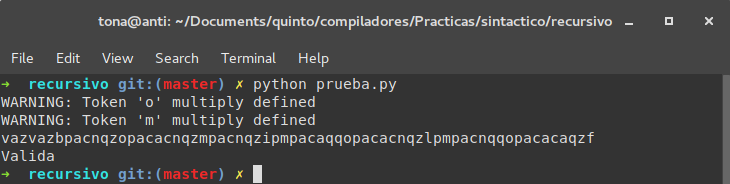
\includegraphics[width=15cm]{prueba1.png}
    \caption{Prueba 1 sobre un archivo bien estructurado.}
    \label{fig:prueba1}
    \end{center}
\end{figure}
Ahora, el archivo que se introdujo en la prueba 1 se modifico para que 
presentara algunos errores por lo que el analizador sintáctico desarrollado 
debería de indicar que el archivo de entrada no es valido, cosa que sucede como 
se muestra en la figura \ref{fig:prueba3} por lo que podemos concluir que 
funciona correctamente. El archivo modificado que se use esta vez fue el 
siguiente.
\begin{lstlisting}
var hola;
var temp

asig(id, 5);
sumar(id, id 7);

mayorque(id, 8);

if (mayorque(id, i)
    restar(id, id, 7);
while (menorque(id, 777))
    sumar(id, id, id);

eof
\end{lstlisting}
En este archivo, se removieron símbolos como punto y coma, paréntesis y algunas 
comas por lo que el analizador sintáctico imprima que no es valido.

\begin{figure}[H]
    \begin{center}
    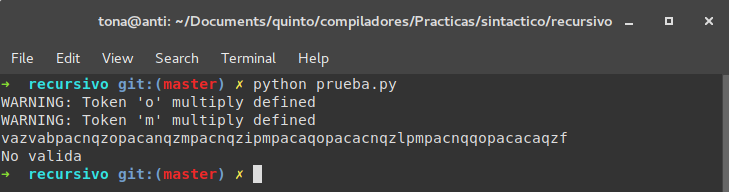
\includegraphics[width=15cm]{prueba2.png}
    \caption{Prueba 2 sobre un archivo con errores.}
    \label{fig:prueba2}
    \end{center}
\end{figure}
\section{Conclusiones}
El analizador sintáctico por descenso recursivo es bastante sencillo por lo que 
es fácil entender el como funciona es por esto que para ejemplos como el 
trabajado en esta 
practica es bastante útil debido a que la gramática también es simple, esto se 
ve 
reflejado en el hecho de que la parte más difícil de esta práctica fue definir 
una correcta gramática que permitiera modelar el lenguaje que se trabajo y el 
resto fue abstraer dicha gramática a nivel programación.
\\\\
Sin embargo, al trabajar con ejemplos más complejos este tipo de analizador 
sintáctico no sera tan conveniente debido a las limitaciones que presenta para 
su correcto funcionamiento como lo es el hecho que una gramática que sea 
recursiva por la izquierda puede provocar que se entre en un bucle infinito 
debido a que si nos encontramos una producción que intente expandir un símbolo 
no terminal \emph{A} al tener dicha recursión nos volveremos a encontrar con la 
situación de expandir otra vez a \emph{A}.
A pesar de esto el conocer como funciona permite entender el funcionamiento del 
resto de analizadores sintácticos y el porque se su existencia.
\bibliography{reporte} 
\bibliographystyle{ieeetr}

\end{document}
